\chapter{Introduzione}

Expiration Date è un'applicazione nata per permettere la gestione completa di tutto ciò che riguarda i prodotti alimentari; con essa è infatti possibile gestire gli aspetti relativi:
\begin{itemize}
  \item alla lista della spesa (prodotti che si desidera acquistare)
  \item alla dispensa (prodotti già posseduti)
  \item alle ricette
\end{itemize}

\begin{figure}[H]
  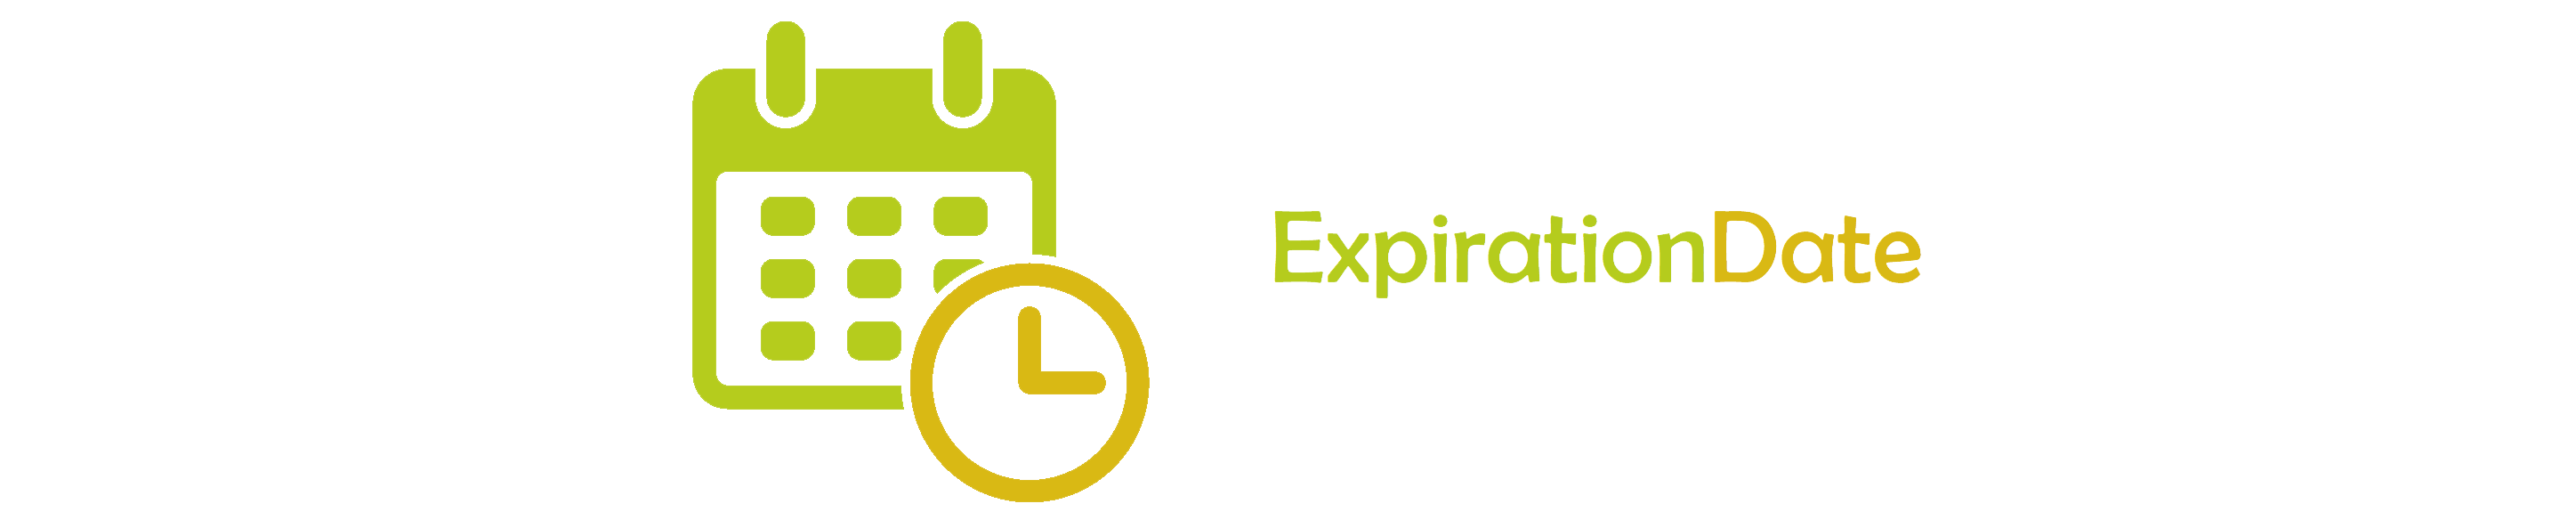
\includegraphics[width=\linewidth]{images/app-logo.png}
  \caption{Logo dell'applicazione.}
  \label{fig:applogo}
\end{figure}

Nel seguito verranno illustrati:
\begin{itemize}
\item i requisiti (funzionali e non funzionali) alla base dello sviluppo dell'applicazione
\item una panoramica generale dell'applicazione, con particolare attenzione all'interfaccia grafica
\item i diagrammi UML (Unified Modeling Language) che descrivono nel dettaglio le funzionalità dell'applicazione e la sua business logic
\item i design patterns implementati, le motivazioni e i vantaggi del loro impiego
\item la tecnica ORM (Object-Relational Mapping) per la gestione della persistenza dei dati e l'interfacciamento con il database
\end{itemize}

\section{Perché Expiration Date?}

Expiration Date è stata la prima applicazione partorita autonomamente dall'inizio alla fine, con ampià libertà decisionale circa le varie scelte progettuali. In particolare, è stata un'opportunità per applicare concetti visti in teoria (e in pratica limitatamente a casi-studio specifici) ad un progetto di proporzioni superiori, favorendone l'assimilazione e accrescendone la padronanza. Ha richiesto l'adozione di punti di vista diversi (quello dell'utente e quello del programmatore), sono state necessarie riflessioni circa quali funzionalità implementare e come implementarle, oltre a dover produrre una documentazione che permettesse anche ad entità terze di comprendere il lavoro svolto. È stata fondamentale anche l'attenzione dedicata alla scrittura di codice mantenibile che favorisse una successiva estensione delle funzionalità, nell'ottica di un progetto non più con finalità esclusivamente didattiche, ma che potesse fungere da ingresso verso quello che è l'effettivo mondo dello sviluppo software, dove l'affidabilità, la stabilità e la durabilità nel tempo costituiscono fattori chiave per il successo di un'applicazione.

\subsection{Perché ORM?}

Quando l'applicazione è stata concepita per la prima volta, senza l'uso di ORM, il tempo speso per gestire le problematiche legate alle differenze (concettuali ma non solo) fra database relazionale e programmazione orientata agli oggetti ha costituito una frazione significativa del tempo totale necessario allo sviluppo: l'unione di SQL e Java richiedeva una conoscenza approfondita di due domini distinti, e il problema della loro inter-operabilità era completamente delegato al programmatore, con conseguente aumento dei tempi sia lato progettazione che lato implementazione e testing. Sfruttando l'ORM come layer intermedio, invece, lo sviluppatore può concentrarsi maggiormente sulla logica applicativa ad alto livello, e anche l'implementazione richiede la conoscenza approfondita di un solo dominio, ovvero quello del linguaggio di programmazione con cui si scrive il codice. Concretamente, l'utilizzo di ORM permette, a parità di tempo, di dotare l'applicazione di molte più funzionalità e di condurre un testing più approfondito ed affidabile; oppure, a parità di funzionalità e di testing, di risparmiare una quantità considerevole di tempo. Inoltre, in un'ottica di estendibilità e stabilità dell'applicazione nel tempo, l'adozione di ORM e la conseguente astrazione che esso offre, permette di separare agevolmente dettagli implementativi di basso livello (come la scelta del database da utilizzare) dalla logica di business dell'applicazione, consentendo modifiche ed aggiunte in maniera rapida ed efficiente garantendo il funzionamento costante dell'applicazione. Concretamente, questo riduce notevolmente lo sforzo necessario per adottare al posto di MySQL, usato per la versione desktop dell'applicazione, SQLite per un'eventuale versione mobile. Maggiori dettagli sui vantaggi di ORM verranno forniti nella sezione corrispondente. 
